\documentclass[book.tex]{subfiles}
\begin{document}
This chapter describes the target hardware of Wolfenstein 3D. For simplicity it is abstracted as a pipeline taking user commands as entry and outputting images and audio at hopefully result into fun things.

\begin{figure}[H]
\centering
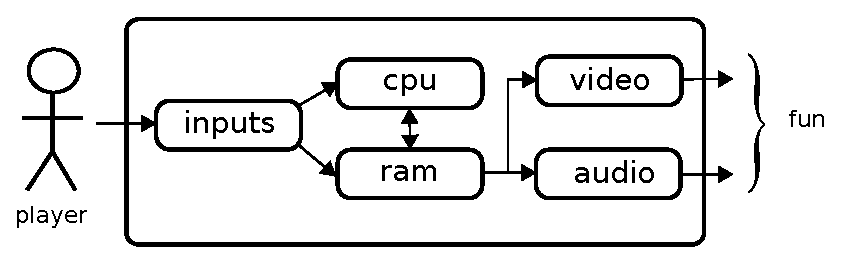
\includegraphics[scale=0.7]{imgs/fun_pipeline.eps}
%\def\svgscale{1.5}
%\input{imgs/fun_pipeline.pdf_tex}
\caption{Hardware pipeline.}
\label{fig:digraph}
\end{figure}

The pipeline comprises five stages. Some of them are bottlenecks for 3D game development while some are surprisingly good:

 \bigskip

\begin{figure}[H]
\centering
\begin{tabularx}{\textwidth}{ X X  }
  \toprule
  \textbf{Stage} & \textbf{Quality} \\ \bottomrule
  CPU & Poor \\ 
  RAM & Very Poor \\ 
  Video & Poor \\ 
  Audio & Good \\ 
  Inputs & Good \\ \bottomrule
\end{tabularx}
\caption{Pipeline stages.}  \label{fig:Pipeline stages}
\end{figure}

Overall, the pipeline offered a lot of resistance: hardware manufacturers had not embraced the game industry yet and it showed a lot. Ever since their inception in the 70s, Personal Computers were designed to display static images and crunch integers. Real-time 3D, fractions and smooth sixty-frames-per-seconds animations were not on the blueprints.

\section{Central Processing Unit}
  \subsection{Landscape}
  The ubiquitous CPU manufacturer was Intel with its x86 line of microprocessors.  The machines based on the 80286 released in 1982 were on the decline and progressively replaced by Intel's first 32 bits processor: The 80386. Moore's law was in full effect as can be seen on a MIPS\footnote{Million Instructions Per Second.} histogram:


\definecolor{skyblue1}{rgb}{0.1,0.624,0.812}


\begin{figure}[H]
\centering
  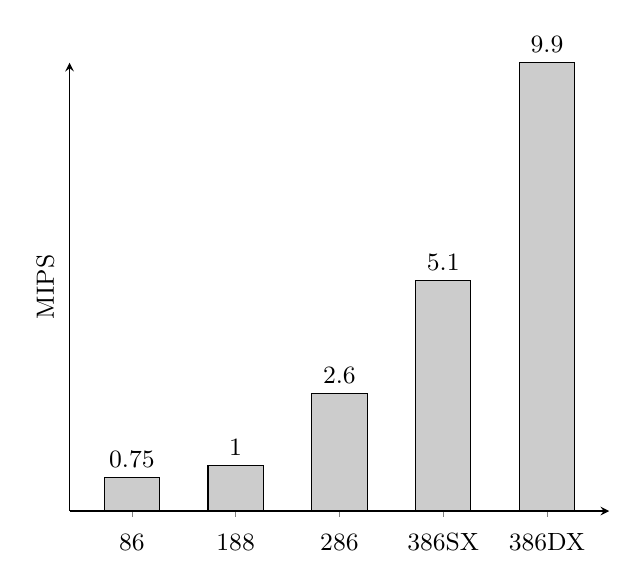
\begin{tikzpicture}[font=\small]
    \begin{axis}[
      ybar,
      bar width=20pt,
      ylabel={MIPS},
      ymin=0,
      ytick=\empty,
      xtick=data,
      axis x line=bottom,
      axis y line=left,
      enlarge x limits=0.15,
      symbolic x coords={86,188,286,386SX,386DX},
      xticklabel style={anchor=base,yshift=-\baselineskip},
      nodes near coords={\pgfmathprintnumber\pgfplotspointmeta}
    ]
      \addplot[fill=black!20,draw=black] coordinates {
        (86,0.75)
        (188,1)
        (286,2.6)
        (386SX,5.1)
        (386DX,9.9)
      };
    \end{axis}
    
   \end{tikzpicture}
   \caption{Processor speeds comparison.} \label{fig:mips}
 \end{figure}

 \textbf{\underline{Trivia :}} A modern processor such as the Intel Core i7 3.33 GHz operates at close to 180,000 Mips: Five orders of magnitude faster!

 \bigskip

\textbf{\underline{Trivia :}}  Two other companies were producing Intel clones: AMD and Cyrix. The mediocre performances did not justify the lower cost and as a result they never gathered a significant market share. Interestingly AMD evolved to become a serious challenger while Cyrix merged with National Semiconductor in 1997.

 \bigskip
 
 \textbf{\underline{Trivia :}} The 386SX and 386DX were identical processor. Yet the DX is twice faster than the SX thanks to a bus twice as wide (32 bits vs 16 bits) !












  \subsection{Floating Point}
  
  Wolfenstein 3D target machines were high-end 286 and low-end 386 machine. As seen previous, those were powerful machines far outperforming any game console on the market. But all that power was not necessarely useful. In order to perform all the trigonometry necessary to perspective effect, the machines had to keep track of the fractional part of each operations. This is usually not an issue since the C language offers the types \codeword{float} and \codeword{double} precisely for that.\\
\\
It is important to understand what floating point is and how it works to fully grasp how useful it is when doing trigonometry. Most of the time it is explained as follow. Take 32 bits and divide them into three parts:

\begin{figure}[H]
\centering
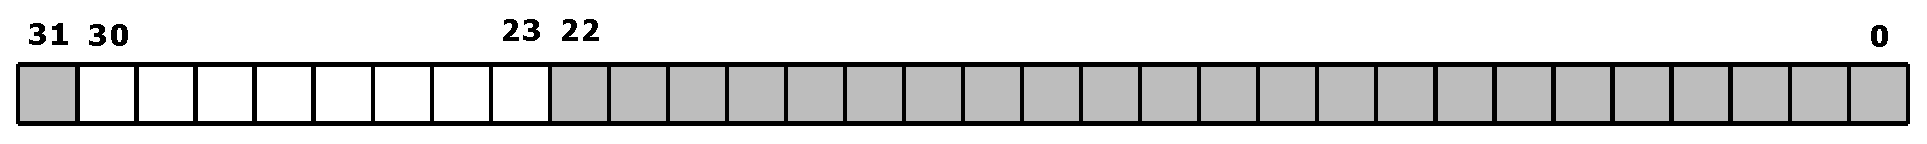
\includegraphics[scale=0.4]{imgs/floating_point_layout.eps}
\caption{Floating Point internals}
\label{fig:fp_internals}
\end{figure}
  \bigskip

\begin{itemize}
  \item One bit S for the sign.
  \item Seven bits E for the exponent.
  \item Twenty four bits for the mantissa.
\end{itemize}  

\begin{figure}[H]
\centering
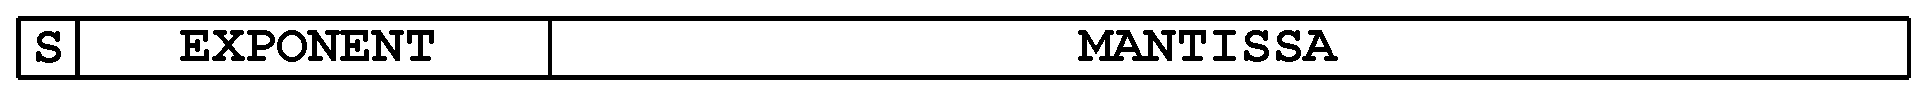
\includegraphics[scale=0.4]{imgs/floating_point_math.eps}
\caption{Floating Point internals}
\label{fig:fp_internals}
\end{figure}
  \bigskip  


Those three parts are usually explained by text books with formula \ref{eq:fp}.\\


\begin{equation}\label{eq:fp}
\large
(-1)^S * 1.M * 2^{(E-127)}
\end{equation}
 
\bigskip  

Which I personnaly hate and find cryptic. I personnaly blame this notation for discouraging generations of programmers, scaring them to never look back and really understand how it works. There is a better way to explain it with a nice drawing and a slightly difference approach. Instead of Exponent, think of a floating window between two consecutive power of two. And instead of a Mantissa think of an Offset within that window as in Figure \ref{fig:fp_internals}:
  
\begin{figure}[H]
\centering
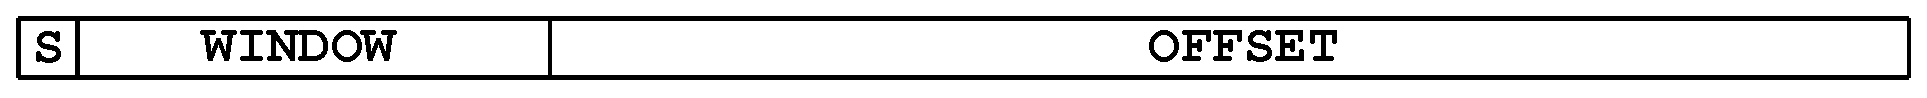
\includegraphics[scale=0.4]{imgs/floating_point_intuitive.eps}
\caption{Floating Point internals}
\label{fig:fp_internals}
\end{figure}
  \bigskip  

Figure \ref{fig:fp_internals_window} illustrate how the number 6.7 would be encoded, with the window starting at 4 (and therefore spanning up to next power of two: 8). The offset about 3/4 along the window.

\begin{figure}[H]
\centering
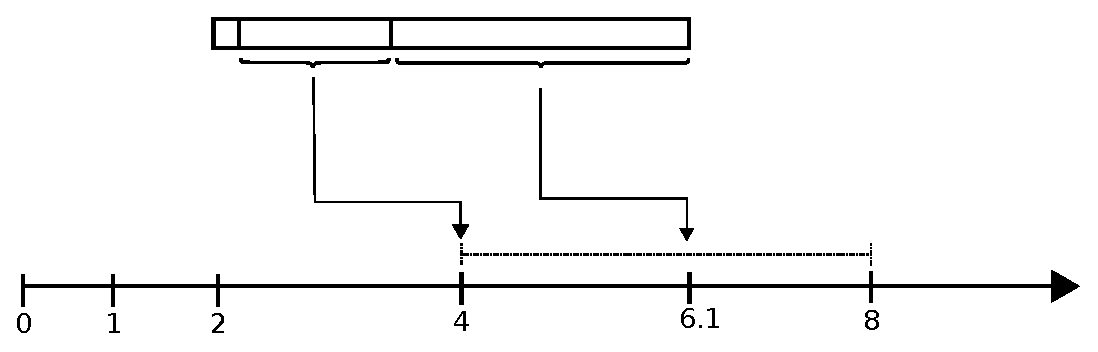
\includegraphics[scale=0.7]{imgs/floating_point_window.eps}

\caption{Floating Point internals}
\label{fig:fp_internals_window}
\end{figure}
  \bigskip
  
Here is a detailled example which calculate the floating point representation of the number 3.14.
\begin{itemize}
 \item The number is positive  $\rightarrow S=0$.
 \item The number is between the power of two 2 and 4 so the floating window must start at $2^1$  $\rightarrow E=128$.
 \item Finally there are $2^{23}$ offsets available so 3.14 is at $\frac{4-3.14}{2} = 0.43 $. The mantissa/offset $\rightarrow M = 2^{23}*0.43 = 4781506$
\end{itemize}

Which in binary translate to:

\begin{itemize}
\item S = 0.
\item E = 10000000
\item M = 1001000111101111000011
\end{itemize}

\begin{figure}[H]
\centering
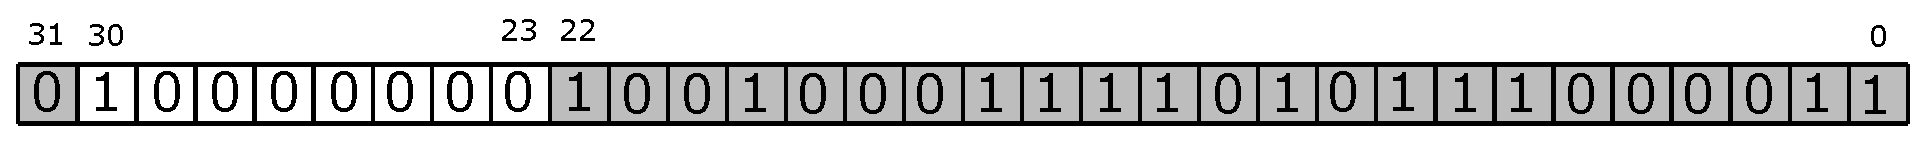
\includegraphics[scale=0.4]{imgs/floating_point_layout_pi.eps}
\caption{Floating Point internals}
\label{fig:fp_internals}
\end{figure}
  \bigskip

The value 3.14 is best approximated as 3.140000104904175.\\

The corresponding value with the ugly and useless formula:

\begin{equation}
3.14 = (-1)^0 * 1.57 * 2^{(128-127)}
\end{equation}

\bigskip

And finally the graphic representation:\\

\begin{figure}[H]
\centering
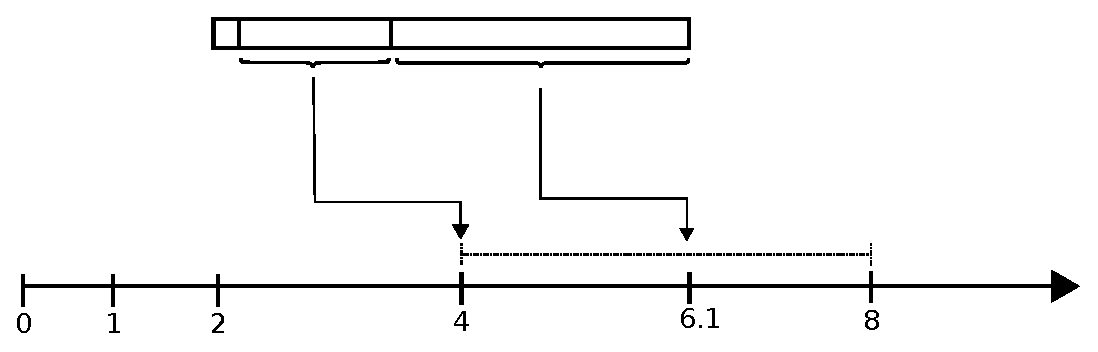
\includegraphics[scale=0.7]{imgs/floating_point_window.eps}

\caption{3.14 window and offset.}
\label{fig:fp_internals}
\end{figure}
  \bigskip

If you understand Floating Point, you can understand how handy it is to a 3D engine.
Not only it approximate number very well, it also protect from overflow by floating floating the window when necessary.\\
\\
The representation is neat but performing operation are inherently computational intensive. In order to add, substract,multiply or divide two numbers, operations have to be carried at a higher precision than 32 bits (80 bits in Intel CPU). With 16 bits registers you can easily understand the gynmastic necessary. On top of that, the representation have to be modified in order to use the same floating window.
\\
This is not a problem when everything is hardwired...but it was a big problem for the 286 and the 386: \emph{They did not have a hardware Floating Point Unit}. Those operations were emulated in software by the compiler and therefore impossibly slow. At first sight it looked like fractions and 3D were out of the picture. A workaround had to be found.

  \bigskip

 \textbf{\underline{Trivia :}} Since floating point units where so rare, why did the C language end up with a \codeword{float} type ? The machine used to invent it (PDP-11) did not have one either but the manufacturer (DEC) had promised Dennis Ritchie and Ken Thompson the next model would have one\footnote{The Development of the C Language by Dennis M. Ritchie}!

\textbf{\underline{Trivia :}} Intel did offer FPUs. Show image here.

At first sight, \emph{int} were fast but not accurate enough and \emph{float} were accurate but not fast enough. It looked like there was not way to do real-time trigonometry.

   















\section{RAM}
The goal of the CPU stage was to manipulate values in RAM. The target machines had an address bus 32 bits wide with a MMU\footnote{Memory management Unit} offering up to 4 GB of linear RAM in Protected Mode. Unfortunately, there was a major obstacle between the programmer and the machine. It was the operating system and its name was MS-DOS 5.0 by Microsoft Corporation.
  






  \subsection{DOS limitations}
DOS 5.0 was released by Microsoft in 1991. It was the \emph{de-facto} operating system that came with every machine sold. It was universal and unavoidable. Since Microsoft was extremely protective of its software base, it was fully backward compatible with previous versions. Which mean it kept the CPU in Real Mode: An abomination that matched the early 
Intel 8086 CPU from 1976.

\bigskip

 \textbf{\underline{Trivia :}} One year earlier, in 1991, a student from Finland started working on a "hobby" of his: An operating system able to use the CPU in Protected Mode. It was Linus Torvalds starting what would become Linux.



  \subsection{16 bits Segmented RAM}
  Real-Mode was the way RAM was layed out in 1976: A 20 bits wide address bus offering up to 1MB of RAM. No matter how much memory was installed on the machine in 1992, only 1MB could be addressed. Addressing was done by combining 16 bits register together. One being a segment, the other the offset within that segment. Hence the name: '16 bits programming'.

  \bigskip

Figure \ref{fig:RealMode_RAM_layout} shows the area in the 1MB:
  \begin{itemize}
  

\item From 0 to 3FFh was the Interrupt Vector Table.
\item From 400h to 4FFh was BIOS data.
\item From 500h to 5FFh was command.com+io.sys.
\item From 600h to 9FFFFh  was the game program. 
\item From A0000h to FFFFFh was a zone called UMA (Upper Memory Area): Reserved to bios ROM, video card and sound card mapped I/O.
\end{itemize}

Out of 1024KB only 640KB (the Conventional Memory) were usable since 384KB were reserved for the UMA. The more drivers (.SYS and .COM) an user loaded on a system at startup, the less was available for the game.

\bigskip

\textbf{\underline{Trivia :}}  In France people had to load KEYBFR.SYS driver so their AZERTY keyboard would work properly. That driver consumed a whopping 5KB.

  \begin{figure}[H]
\centering
 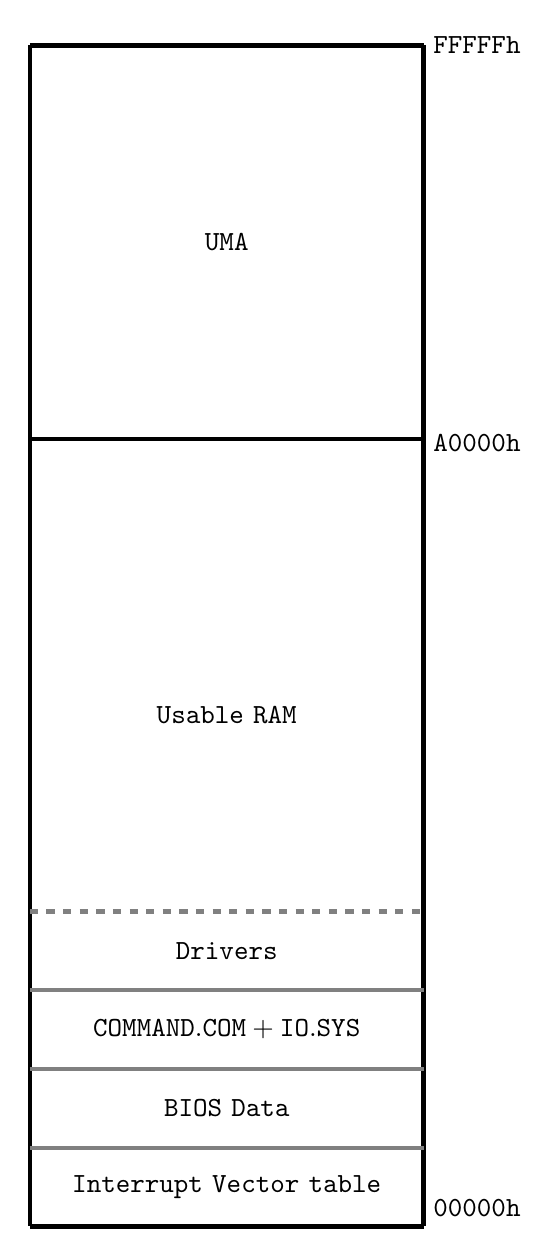
\begin{tikzpicture}


%Draw borders of ALL RAM
\draw[ultra thick,black] (5,0)  -- (0,0);
\draw[ultra thick,black] (5,0 ) -- (5,15);
\draw[ultra thick,black] (0,15) -- (5,15);
\draw[ultra thick,black] (0,15)  -- (0,0);

%Defining grey color
\colorlet{LighterMark}{black!50}

%Interrupt Vector table
\draw[ultra thick,LighterMark] (0,1)  -- (5,1);
\node[] at (2.5,0.5){$\mathtt{Interrupt\ Vector\ table}$}  ;


\node[above right,align=left] at (5,0){$\mathtt{00000h}$}  ;

%BIOS data
\draw[ultra thick,LighterMark] (0,2)  -- (5,2);
\node[] at (2.5,1.5){$\mathtt{BIOS\ Data}$}  ;

%COMAMND.COM + IO.SYS
\draw[ultra thick,LighterMark] (0,3)  -- (5,3);
\node[] at (2.5,2.5){$\mathtt{COMMAND.COM + IO.SYS}$}  ;

%Drivers
\draw[ultra thick,dashed,LighterMark] (0,4)  -- (5,4);
\node[] at (2.5,3.5){$\mathtt{Drivers}$}  ;

%Usable RAM
\node[] at (2.5,6.5){$\mathtt{Usable\ RAM}$}  ;

%UMA
\draw[ultra thick,black] (0,10)  -- (5,10);
\node[right,align=left] at (5,9.95){$\mathtt{A0000h}$}  ;
\node[] at (2.5,12.5){$\mathtt{UMA}$}  ;

%Top RAM
\node[right,align=left] at (5,15){$\mathtt{FFFFFh}$}  ;

%Braces
%\draw [decorate,decoration={brace,amplitude=10pt,mirror,raise=4pt},yshift=0pt]
%(5,0) -- (5,10) node [black,midway,xshift=0.8cm] {\footnotesize
%$XXXX$};

\end{tikzpicture}
 \caption{RealMode RAM layout.} \label{fig:RealMode_RAM_layout}
 \end{figure}




It gets worse. Since two 16 bits register were combined to form a RAM address, two pointers could point to the same RAM location but fail an equality test:
\bigskip
With pointer A defined as:
\begin{Verbatim}[fontsize=\relsize{-1}]
    0110 1000 1000 0111 0000  Segment, 16 bits shifted 4 bits left  
  +      0011 0100 1010 1001  Offet,   16 bits
============================
    0110 1011 1101 0001 1001  Address, 20 bits
\end{Verbatim}

\bigskip

Pointer B defined as:
\begin{Verbatim}[fontsize=\relsize{-1}]
    0000 0000 0001 0000 0000  Segment, 16 bits shifted 4 bits left  
  +      0000 0000 0010 0000  Offet,   16 bits
============================
    0000 0000 0001 0010 0000  Address, 20 bits
\end{Verbatim}

\bigskip

Pointer C defined as:
\begin{Verbatim}[fontsize=\relsize{-1}]
    0000 0000 0001 0010 0000  Segment, 16 bits shifted 4 bits left  
  +      0000 0000 0000 0000  Offet,   16 bits
============================
    0000 0000 0001 0010 0000  Address, 20 bits
\end{Verbatim}

As defined A, B and C all points to the same memory location but however would fail a comparison test in the following code.\\

\begin{Verbatim}[fontsize=\relsize{-1}]
far void* a = FP_SEG(0x0000) + FP_OFF(0x0120);
far void* b = FP_SEG(0x0010) + FP_OFF(0x0020);
far void* c = FP_SEG(0x0012) + FP_OFF(0x0000);
\end{Verbatim}

\bigskip

\begin{Verbatim}[fontsize=\relsize{-1}]

a == b  -> false
a == c  -> false
b == c  -> false
\end{Verbatim}

\bigskip

{\underline{Trivia :}} The 640KB barrier was so complex that id Software provided a special tech suport executable: w3dhelp.exe which provides extensive description of the 640KB barrier\footnote{You can read it in the annexe \ref{640barrier} of this book.}.

\bigskip

{\underline{Trivia :}} The original C language did not have near and far keyboard because the PDP computer they worked with had 32 bits registers and MMU (Memory Managment Unit) that make the RAM appear linear even within a process.




  \subsection{Extended Memory}

In Real-Mode the processor could access 1MB no matter what. But machines of 1992 can equipped with up to 2MB. 

  \begin{figure}[H]
\centering
 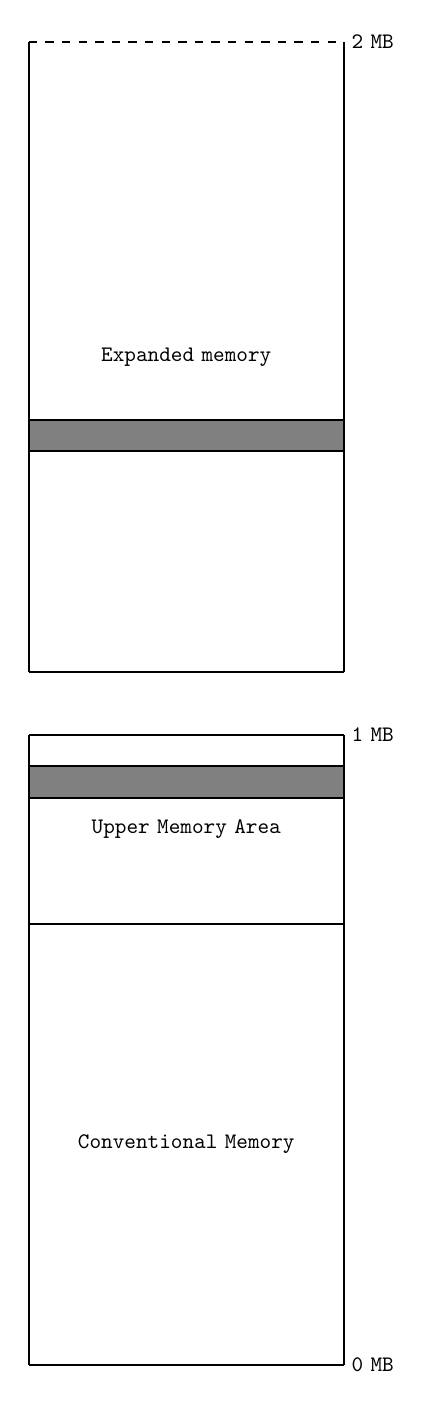
\begin{tikzpicture}[scale=0.8, every node/.style={scale=0.8}]

%Draw borders of ALL RAM
\draw[thick,black] (5,0)  -- (0,0);
\draw[thick,black] (5,0 ) -- (5,10);
\draw[thick,black] (0,10) -- (5,10);
\draw[thick,black] (0,10)  -- (0,0);

%Defining grey color
\colorlet{LighterMark}{black!50}

\node[right,align=left] at (5,0){$\mathtt{0\ MB}$}  ;

%UMA
\draw[thick,black] (0,7)  -- (5,7);

%Top RAM
\node[right,align=left] at (5,10){$\mathtt{1\ MB}$}  ;

\draw[thick,black] (5,11)  -- (0,11);
\draw[thick,black] (5,11 ) -- (5,21);
\draw[thick,black,dashed] (0,21) -- (5,21);
\draw[thick,black] (0,21)  -- (0,11);
\node[right,align=left] at (5,21){$\mathtt{2\ MB}$}  ;

\draw [thick,fill=LighterMark] (0,9) rectangle (5,9.5);
\draw [thick,fill=LighterMark] (0,14.5) rectangle (5,15);

\node[] at (2.5,3.5){$\mathtt{Conventional\ Memory}$}  ;
\node[] at (2.5,16){$\mathtt{Expanded\ memory}$}  ;
\node[] at (2.5,8.5){$\mathtt{Upper\ Memory\ Area}$}  ;

\end{tikzpicture}

 \caption{Extended Memory.}
 \end{figure}


{\underline{Trivia :}}  As of 2014, thirty five years after the introduction of the 8086, most PC in the world start in  real mode. Then a bootloader switch them to protected mode, load the kernel and then real startup can begin. Mac computers don’t have this problem.

\bigskip

{\underline{Trivia :}}  As of 2014, thirty five years after the introduction of the 8086, most PC in the world still use segmented addressing.




\section{Video}

PC were connected to a CRT monitor: Huge, cathodic ray based, small screen, curved surface, deep and incredibly heavy devices. Most had a tiny 13” diagonal and all had a 4:3 ratio. Figure \ref{fig:int_layout} shows a comparison with a 28” LCD display from 2014.

  \begin{figure}[H]
\centering
 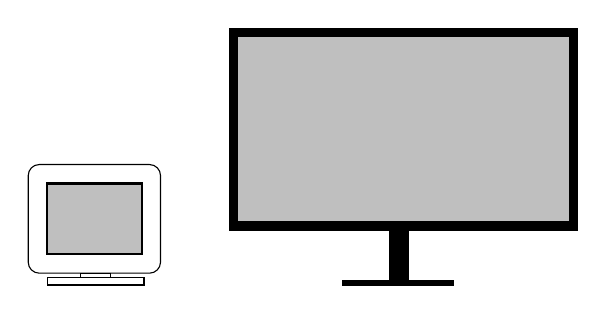
\begin{tikzpicture}[scale=0.3]

%Defining grey color
\colorlet{LighterMark}{black!25}

%CRT
\draw [thick,fill=LighterMark] (4,5) rectangle (8,8);
\draw [rounded corners] (3.2,4.2) rectangle (8.8,8.8);
\draw [] (5.4,4.2) rectangle (6.7,4);
\draw [] (4,4) rectangle (8.1,3.7);

%LCD
% cadre
\draw [ultra thick,fill=black] (11.8,6.1) rectangle (26.4,14.5);
%active screen
\draw [ultra thick,fill=LighterMark] (12,6.3) rectangle (26.2,14.3);
%bar
\draw [fill=black] (18.5,6.3)    rectangle (19.3,3.7);
%socle
\draw [fill=black] (16.5,3.7) rectangle (21.2,3.9);

\end{tikzpicture}

 \caption{Comparaison CRT vs LCD.}\label{fig:lcd_vs_crt}
 \end{figure}

{\underline{Trivia :}} How big and heavy could a CRT be ? Integraph InterView 28hd96 weighted 45kg (99.5lb). Compared to 7.8kg (17lb). Used for Doom 3 ?! Details about pictures.
\bigskip
The VGA (Video Graphic Array) was the chipset in charge of interfacing the CPU and the CRT:
\bigskip
DRAWING
\bigskip
That chip was a blessing and a curse: It was universally deployed on every single IBM PC on the market but it was also poorly documented and complicated to program with more than 300 internal registers.



  \subsection{History}

The VGA\footnote{Video Graphic Adapter} was the chip interfacing between the PC RAM and the CRT\footnote{Cathode Ray Tube} screen. Released in 1987, it was installed on every single machine on the market. 

\bigskip
  
 \begin{figure}[H]
\centering  
\begin{tabular}{ l | c | l }
  \toprule
  \textbf{Name} &  \textbf{Year Released} \\
  \toprule \codeword{MDA}
   (\textbf{M}onochrome
   \textbf{D}isplay
   \textbf{A}dapater) & 1981 
   \\ \codeword{CGA}
   (\textbf{C}olor
   \textbf{G}raphics
   \textbf{A}dapter) & 1981 
    \\ \codeword{EGA}
   (\textbf{E}nhanced
   \textbf{G}raphics
   \textbf{A}dapter) & 1985
   \\ \codeword{VGA}
   (\textbf{V}ideo
   \textbf{G}raphics
   \textbf{A}rray)  & 1987
    \\
  \toprule
\end{tabular}
\caption{Video interface history.}\label{fig:vga_history}
\end{figure}

The universality of VGA was a two edged sword. One one side, developers did not have to deal with hereogeneity. One the other side, the shortcoming of the Adapater were the same for everybody.




\subsection{VGA Architecture}

  Four parts were interacting around 256Kb of RAM:

\begin{itemize}
\item The Graphic Controller and Sequence Controller controlled how the RAM was populated.
\item The Sequence Controller
\item The CRTC Controller and the DAC (Digital To Analog Converter) took care of sending the content of the RAM to the monitor.
\item The DAC
\end{itemize}

 \begin{figure}[H]
\centering
 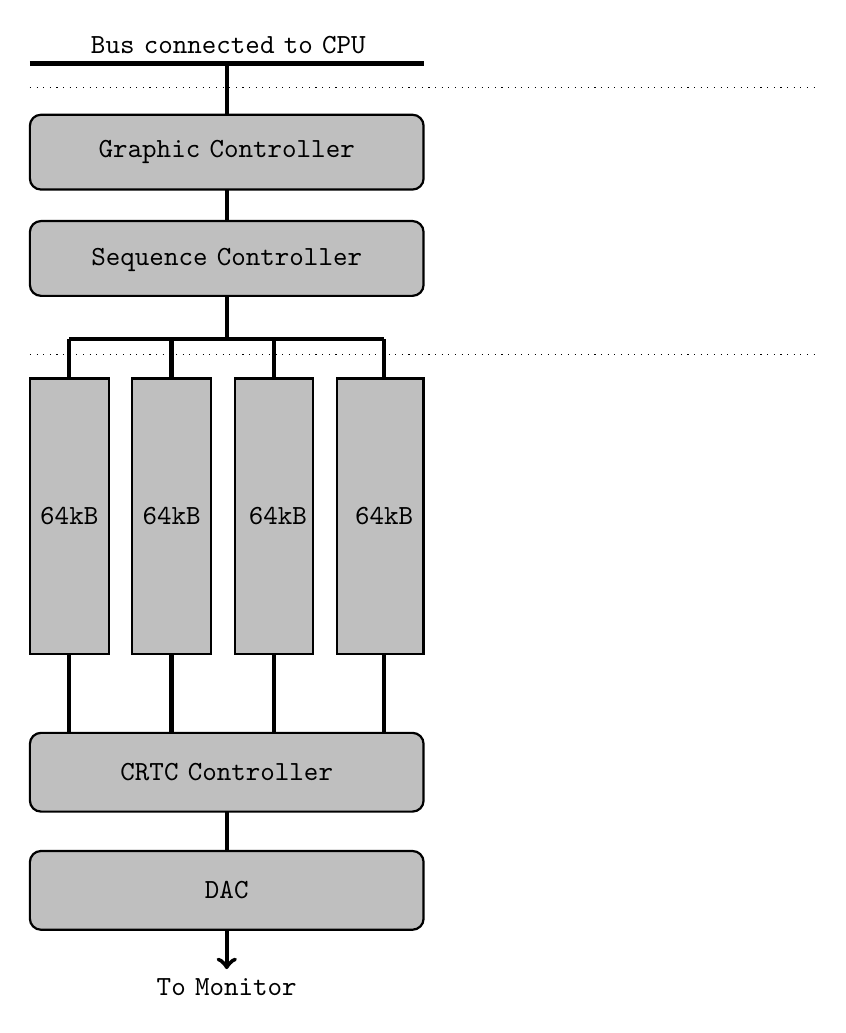
\begin{tikzpicture}

%Defining grey color
\colorlet{LighterMark}{black!25}

\def\planeWidth{2}% plane width
\def\planeHeight{4}% plane height
\def\firstBank{0}
\def\planeSpace{0.1}

%Bus
\draw[ultra thick] (0,15.5) -- (5,15.5);
\node[above] at (2.52,15.5){$\mathtt{Bus\ connected\ to\ CPU}$}  ;

\draw [thick,fill=LighterMark,rounded corners] (0,14.85) rectangle (5,13.9);
\node[] at (2.5,14.375){$\mathtt{Graphic\ Controller}$}  ;

\draw [thick,fill=LighterMark,rounded corners] (0,13.5) rectangle (5,12.55);
\node[] at (2.5,13){$\mathtt{Sequence\ Controller}$}  ;

\draw [thick,fill=LighterMark] (0,11.5)   rectangle (1,8);
\node[] at (0.5,9.75){$\mathtt{64kB}$}  ;

\draw [thick,fill=LighterMark] (1.3,11.5) rectangle (2.3,8);
\node[] at (1.8,9.75){$\mathtt{64kB}$}  ;

\draw [thick,fill=LighterMark] (2.6,11.5)   rectangle (3.6,8);
\node[] at (3.15,9.75){$\mathtt{64kB}$}  ;

\draw [thick,fill=LighterMark] (3.9,11.5)   rectangle (5,8);
\node[] at (4.5,9.75){$\mathtt{64kB}$}  ;

\draw [thick,fill=LighterMark,rounded corners] (0,7) rectangle (5,6);
\node[] at (2.5,6.5){$\mathtt{CRTC\ Controller}$}  ;

\draw [thick,fill=LighterMark,rounded corners] (0,4.5) rectangle (5,5.5);
\node[] at (2.5,5){$\mathtt{DAC}$}  ;

%Connect everything

% bus to GC
\draw[ultra thick] (2.5,15.5) -- (2.5,14.85);

% GC to SC
\draw[ultra thick] (2.5,13.9) -- (2.5,13.5);

% SC to RAM
\draw[ultra thick] (2.5,12) -- (2.5,12.55);

% RAM multiplexer
\draw[ultra thick] (0.5,12) -- (4.5,12);
\draw[ultra thick] (0.5,12) -- (0.5,11.5);
\draw[ultra thick] (1.8,12) -- (1.8,11.5);
\draw[ultra thick] (3.1,12) -- (3.1,11.5);
\draw[ultra thick] (4.5,12) -- (4.5,11.5);

% RAM to CRTC
\draw[ultra thick] (0.5,8) -- (0.5,7);
\draw[ultra thick] (1.8,8) -- (1.8,7);
\draw[ultra thick] (3.1,8) -- (3.1,7);
\draw[ultra thick] (4.5,8) -- (4.5,7);

% CRTC to DAC
\draw[ultra thick] (2.5,6) -- (2.5,5.5);

% CRTC to DAC

\draw[ultra thick,->] (2.5,4.5) -- (2.5,4);
\node[below] at (2.5,4){$\mathtt{To\ Monitor}$}  ;

% Draw text on the side
\draw[dotted] (0,15.2) -- (10,15.2); 


%
\draw[dotted] (0,11.8) -- (10,11.8);


\end{tikzpicture}

 \caption{Video Graphic Array Architecture.}\label{fig:vga_arch}
 \end{figure}

 {\underline{Note :}} The clean pipeline architecture in Figure \ref{fig:vga_arch} is an oversimplication. In reality each Controller interacted with the rest of the system. The Sequece Controller for example could not only interact with the RAM but also gdgdfgegdfg...



The most surprising part of the architecture is the frame buffer (the RAM that contain the image before it is sent to the screen) which is not one big linear array but four parallel memory banks (called planes). The design raison d’etre is twofold :

\begin{itemize}



\item Backward compatibility: EGA (the precursor of VGA) had only 64kB of RAM.
\item Hardware limitations: A CRT running at 60Hz and displaying 640x480 needed a pixel every 1/(640*480*60)th of second . That mean one pixel each 54ns. The problem was the RAM access time was 200ns so that was not possible. But if latency could not be reduced, the throughput could be improved by fetching 1 pixel + 3 others in advance. Therefore the memory banks were read in parallel: 4 bytes at a time and the CRTC had an amortized latency of 200/4 = 50ns/pixel which was fast enough.
\end{itemize}

\bigskip
To help configure automatically the 300 registers of the VGA, the IBM BIOS had a preset number of mode with an associated resolution and color space :

\begin{figure}[H]
\centering
\begin{table}[H]
\begin{tabular}{llllr}
\hline
\textbf{Mode} & \textbf{Type} & \textbf{Format} & \textbf{Colors}          & \multicolumn{1}{l}{\textbf{Segment}} \\ \hline
0             & text          & 40x25           & 16 gradient (monochrome) & b800h                                \\ \hline
1             & text          & 40x25           & 16                       & b800h                                \\ \hline
2             & text          & 80x25           & 16 gradient (monochrome) & b800h                                \\ \hline
3             & text          & 80x25           & 16                       & b800h                                \\ \hline
4             & CGA Graphics  & 320x200         & 4                        & b800h                                \\ \hline
5             & CGA Graphics  & 320x200         & 4 gradient (monochrome)  & b800h                                \\ \hline
6             & CGA Graphics  & 640x200         & 2                        & b800h                                \\ \hline
7             & MDA text      & 9x14            & 3 gradient (monochrome   & b000h                                \\ \hline
0Dh           & EGA graphic   & 320x200         & 16                       & A000h                                \\ \hline
0Eh           & EGA graphic   & 640x200         & 16                       & A000h                                \\ \hline
0Fh           & EGA graphic   & 640x350         & 3                        & A000h                                \\ \hline
10h           & EGA graphic   & 640x350         & 16                       & A000h                                \\ \hline
11h           & VGA graphic   & 640x480         & 2                        & A000h                                \\ \hline
12h           & VGA graphic   & 640x480         & 16                       & A000h                                \\ \hline
13h           & VGA graphic   & 320x200         & 256                      & A000h                                \\ \hline
\end{tabular}
\end{table}
\caption{VGA Modes available from BIOS.}\label{fig:vga_modes}
 \end{figure}
 

\begin{figure}[H]
\centering
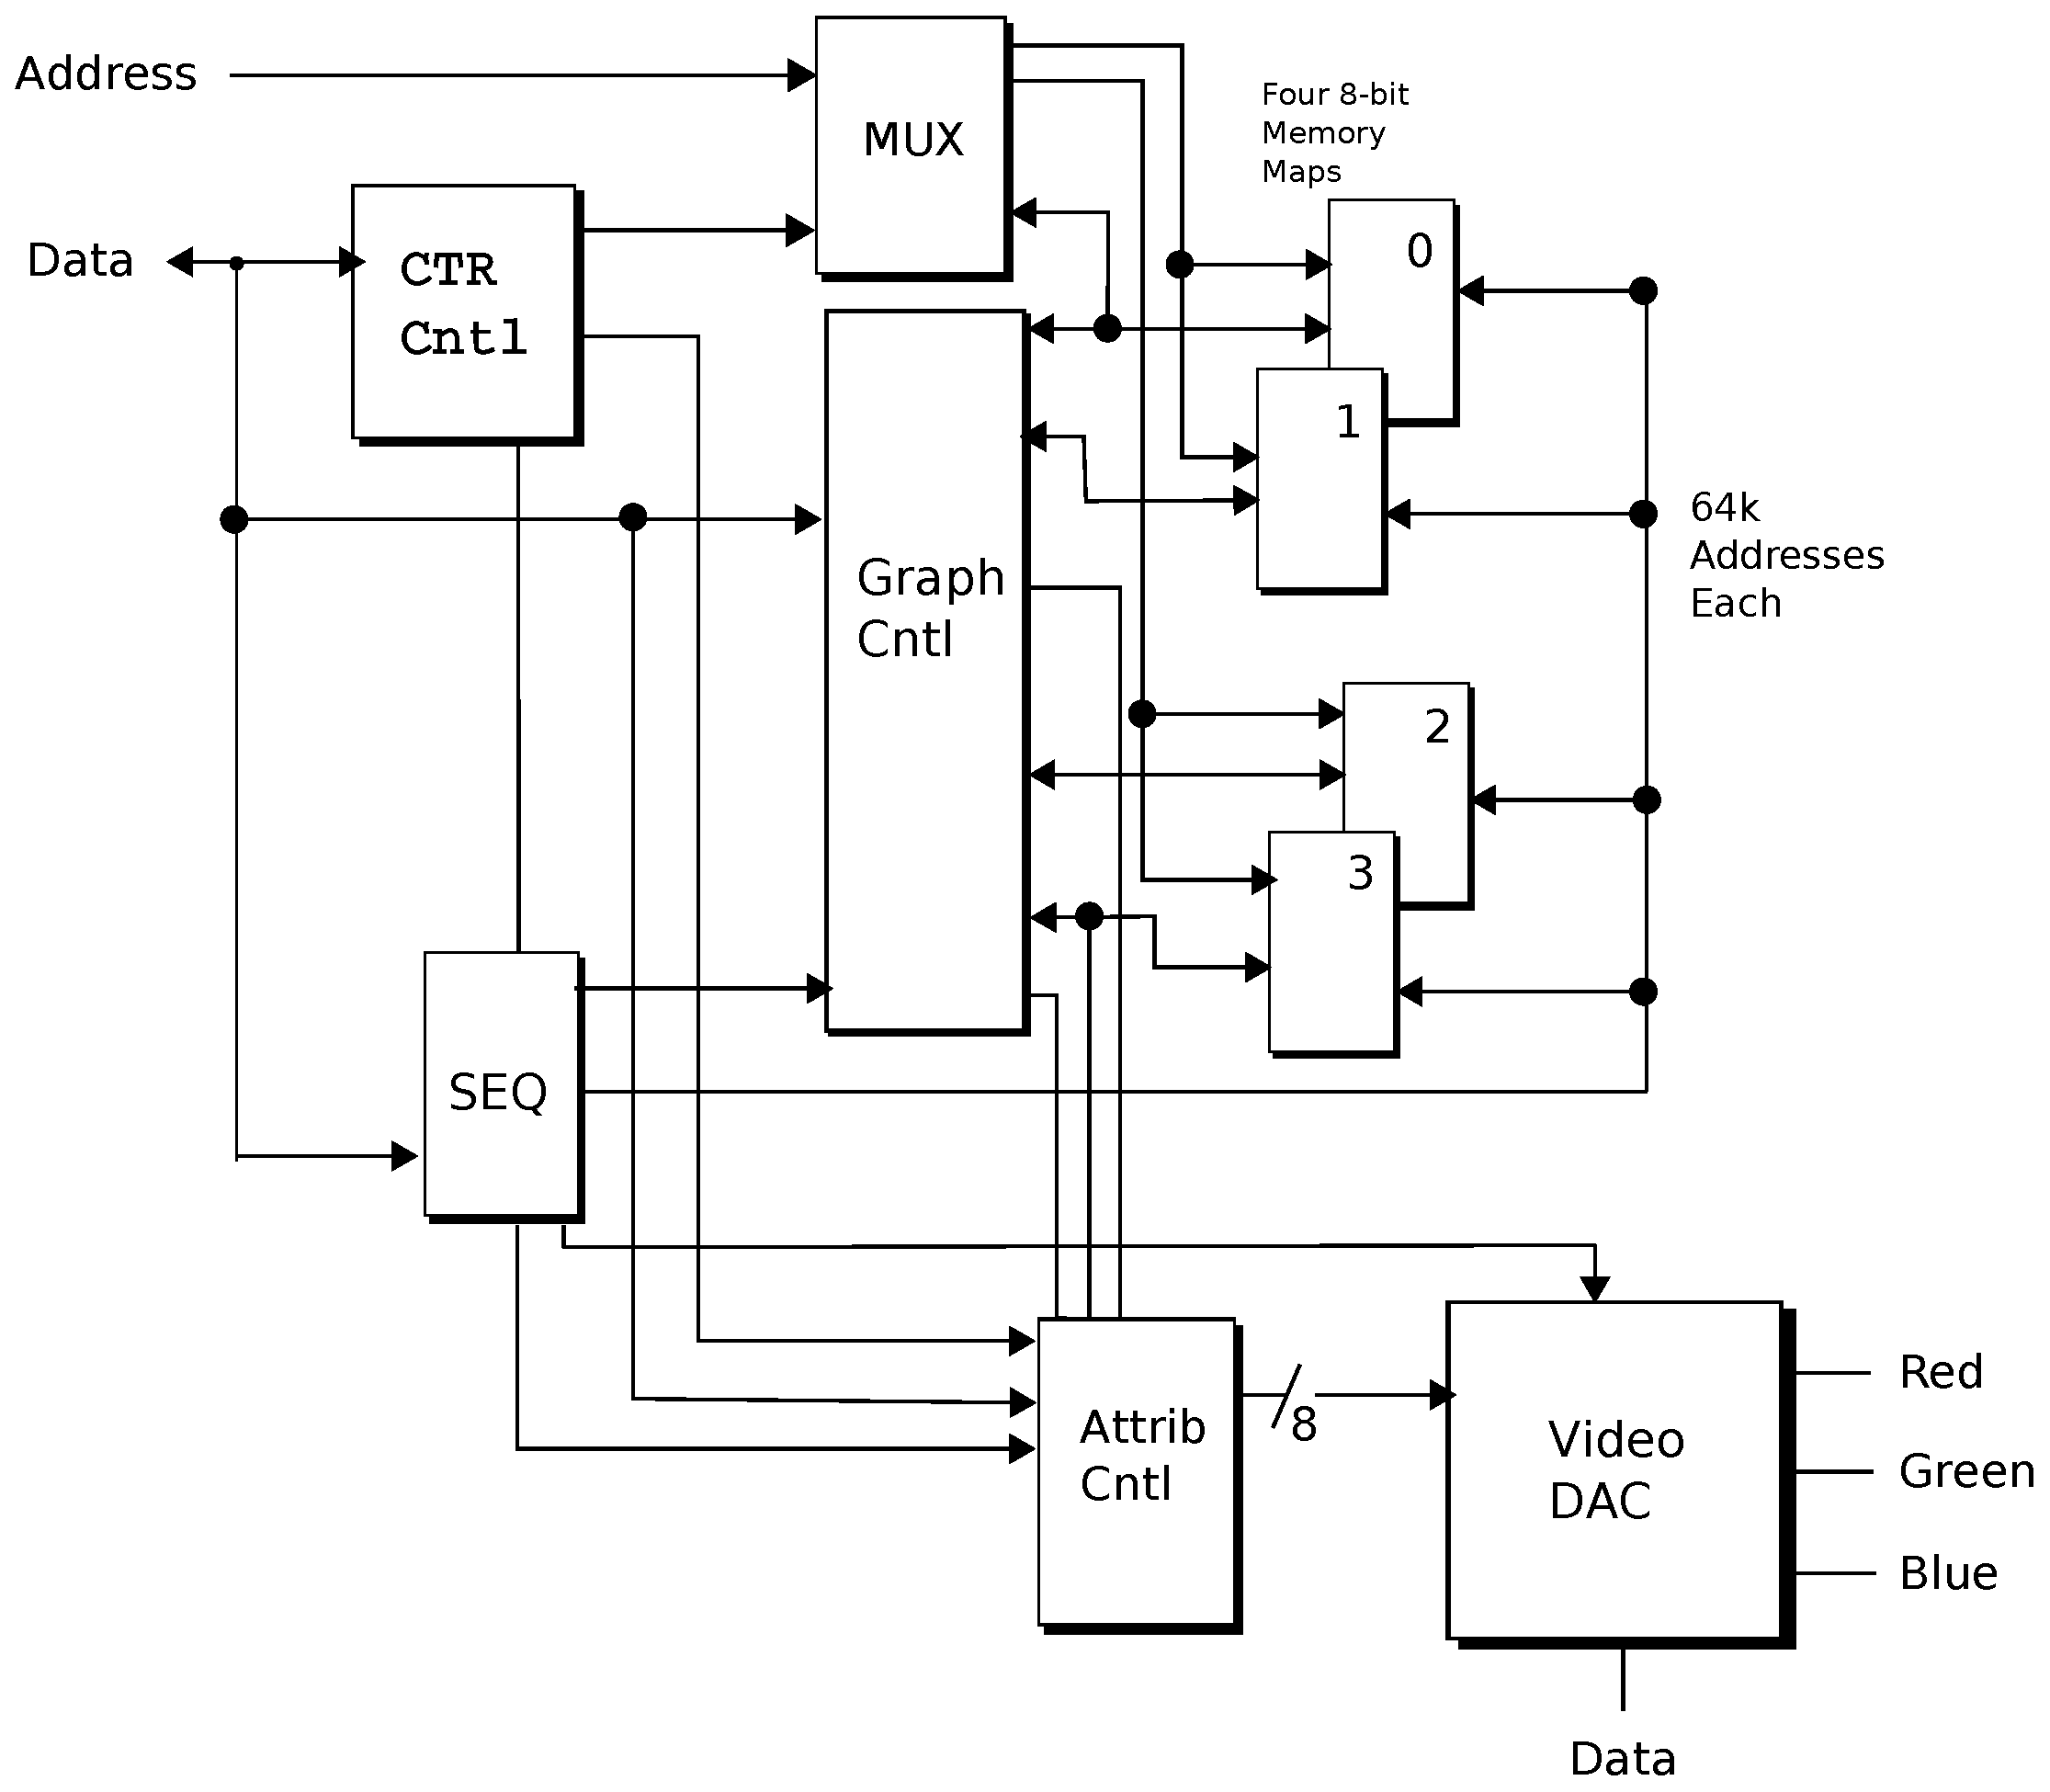
\includegraphics[scale=0.38]{imgs/ibm_vga.eps}
%\def\svgscale{1.5}
%\input{imgs/fun_pipeline.pdf_tex}
\caption{IBM's VGA Documentation}
\label{fig:ibm_vga}
\end{figure}

The VGA was actually a mess. Inside the chip every components were connected to each other and configured via more than 300 registers.\\
\\
Abrash citation about difficulty.
 
 
  \subsection{VGA setup}

  \subsection{VGA Programming}
  \subsection{VGA Mode Y}
\section{Audio}
  \subsection{Speaker}
  \subsection{Ad Lib}
  \subsection{Sound Blaster}

\section{Inputs}

\end{document}




